\documentclass[aspectratio=169,11pt]{beamer}

% Build from the repository root:
% latexmk -pdf -interaction=nonstopmode -halt-on-error \
%   -outdir=docs/build docs/combination_testing_research.tex
% Copy docs/build/combination_testing_research.pdf to docs/.
% All figures are editable vector graphics. No external images are required.

\usepackage[T1]{fontenc}
\usepackage{lmodern}
\usepackage{amsmath,amssymb,mathtools}
\usepackage{booktabs,array}
\usepackage{tikz}
\usetikzlibrary{arrows.meta,positioning,calc,fit}
\usepackage{fontawesome5}
\usepackage{listings}
\newcolumntype{L}[1]{>{\raggedright\arraybackslash}p{#1}}

\definecolor{Navy}{HTML}{172B4D}
\definecolor{Teal}{HTML}{087F8C}
\definecolor{Amber}{HTML}{B66B13}
\definecolor{Red}{HTML}{B54444}
\definecolor{Muted}{HTML}{59677A}
\definecolor{Pale}{HTML}{F2F5F8}
\definecolor{Mint}{HTML}{E8F5F1}
\definecolor{Sand}{HTML}{FFF3DD}
\definecolor{Lavender}{HTML}{EFEAF7}
\definecolor{Purple}{HTML}{7353A6}

\setbeamersize{text margin left=9mm,text margin right=9mm}
\setbeamercolor{normal text}{fg=Navy,bg=white}
\setbeamercolor{frametitle}{fg=Navy,bg=white}
\setbeamercolor{title}{fg=Navy}
\setbeamercolor{structure}{fg=Teal}
\setbeamercolor{block title}{fg=white,bg=Teal}
\setbeamercolor{block body}{fg=Navy,bg=Pale}
\setbeamercolor{block title alerted}{fg=white,bg=Amber}
\setbeamercolor{block body alerted}{fg=Navy,bg=Sand}
\setbeamerfont{title}{size=\LARGE,series=\bfseries}
\setbeamerfont{frametitle}{size=\large,series=\bfseries}
\setbeamerfont{block title}{size=\small,series=\bfseries}
\setbeamerfont{block body}{size=\small}
\setbeamertemplate{navigation symbols}{}
\setbeamertemplate{itemize items}[circle]
\setbeamertemplate{blocks}[rounded][shadow=false]
\setbeamertemplate{frametitle}{%
  \vspace{2mm}\insertframetitle\par
  \vspace{1.5mm}{\color{Teal}\rule{\textwidth}{0.55pt}}\vspace{1mm}}
\setbeamertemplate{footline}{%
  \leavevmode\hbox{%
  \begin{beamercolorbox}[wd=.82\paperwidth,ht=3.8mm,dp=1.6mm,leftskip=9mm]{normal text}
    \scriptsize\color{Muted}Observation-guided combination testing\hspace{4mm}|\hspace{4mm}Research progress, 30 Sep 2026
  \end{beamercolorbox}%
  \begin{beamercolorbox}[wd=.18\paperwidth,ht=3.8mm,dp=1.6mm,rightskip=9mm plus1fil]{normal text}
    \hfill\scriptsize\color{Muted}\insertframenumber\,/\,\inserttotalframenumber
  \end{beamercolorbox}}}

\hypersetup{pdftitle={Observation-Guided Combination Testing for Coding-Agent Patches},
  pdfauthor={Combination Coverage Research},pdfsubject={Research progress and verified DeepSWE examples},
  colorlinks=true,urlcolor=Teal,linkcolor=Navy}
\pdfstringdefDisableCommands{\def\translate#1{#1}}

\lstdefinelanguage{TypeScript}{keywords={const,let,return,if,else,true,false,undefined},
  sensitive=true,comment=[l]{//},morestring=[b]',morestring=[b]"}
\lstset{basicstyle=\ttfamily\scriptsize,keywordstyle=\color{Teal}\bfseries,
  commentstyle=\color{Muted},stringstyle=\color{Purple},showstringspaces=false,
  backgroundcolor=\color{Pale},frame=none,columns=fullflexible,keepspaces=true,
  breaklines=true,tabsize=2,aboveskip=2mm,belowskip=2mm,xleftmargin=2mm,xrightmargin=2mm}

\newcommand{\src}[1]{\par\vfill\vspace{1mm}{\scriptsize\color{Muted}#1\par}}
\newcommand{\takeaway}[1]{\par\vspace{1.5mm}\begin{beamercolorbox}[sep=1.5mm,wd=\textwidth]{block body}\small\textbf{#1}\end{beamercolorbox}}
\newcommand{\badge}[2]{\tikz[baseline=(n.base)]\node[rounded corners=2pt,fill=#1!12,text=#1,inner xsep=5pt,inner ysep=3pt,font=\scriptsize\bfseries](n){#2};}
\newcommand{\yes}{\textcolor{Teal}{\faIcon{check-circle}}}
\newcommand{\pending}{\textcolor{Amber}{\faIcon{exclamation-circle}}}
\newcommand{\icon}[1]{\textcolor{Teal}{\faIcon{#1}}}
\newcommand{\code}[1]{\texttt{#1}}
\newcommand{\Ret}{\textcolor{Teal}{Retained}}
\newcommand{\Rev}{\textcolor{Purple}{Revised}}

\tikzset{box/.style={draw=Teal!45,fill=Pale,rounded corners=3pt,align=center,
  font=\small,inner sep=5pt},arrow/.style={-{Stealth[length=2mm]},thick,draw=Teal},
  uncertain/.style={arrow,dashed,draw=Amber},
  labeltext/.style={font=\scriptsize,text=Muted,align=center}}

\title{Observation-Guided\newline Combination Testing\newline for Coding-Agent Patches}
\subtitle{Program analysis + bounded semantic reasoning}
\author{Research progress report}
\date{30 September 2026}

\begin{document}

% 1 ------------------------------------------------------------------------
\begin{frame}[plain]
  \vspace{5mm}
  {\color{Teal}\large\faIcon{code-branch}\quad Pre-submission validation research}\par
  \vspace{5mm}
  {\usebeamerfont{title}\inserttitle\par}
  \vspace{4mm}
  {\large\insertsubtitle\par}
  \vspace{6mm}
  \badge{Teal}{16/17 development trials detected}\hspace{3mm}
  \badge{Amber}{Unified abstraction still under development}
  \vfill
  \small\insertauthor\hfill\insertdate\par
  \vspace{3mm}
  \scriptsize\color{Muted}Score: completed fresh v3 run; 14 distinct tasks. Detection is not issue resolution.
\end{frame}

% 2 ------------------------------------------------------------------------
\begin{frame}[t]{The problem: a patch passes its validations but remains wrong}
  \small
  \begin{columns}[T,onlytextwidth]
    \begin{column}{.47\textwidth}
      \begin{block}{\faIcon{history}\quad Available before submission}
        \begin{itemize}
          \item Issue and candidate patch.
          \item Repository and full original trajectory.
          \item Tests, scripts, failures and fixes.
        \end{itemize}
      \end{block}
      Replay the historical state to simulate a plugin before submission.
    \end{column}
    \begin{column}{.49\textwidth}
      \begin{alertblock}{\faIcon{bug}\quad Effective validation gap}
        Validations exercise individual behaviors but miss an interaction, or use an unsuitable observation or expectation.
      \end{alertblock}
      \small\textbf{Goal:} add or modify a valid combination test that exposes the submitted patch's defect.
    \end{column}
  \end{columns}
  \takeaway{Intended endpoint: test feedback $\rightarrow$ patch repair $\rightarrow$ hidden-test evaluation. This repair loop is not yet evaluated.}
  \src{Setting: DeepSWE replay; original trajectory is allowed input. Hidden tests and reference patches are evaluation-only.}
\end{frame}

% 3 ------------------------------------------------------------------------
\begin{frame}[t]{Real DeepSWE failure: HTTPX streaming JSON (N01)}
  \small\textbf{Issue:} incremental JSON iteration must reject malformed data and close a consumed streaming response.
  \vspace{3mm}
  \begin{columns}[T,onlytextwidth]
    \begin{column}{.56\textwidth}
      \renewcommand{\arraystretch}{1.6}
      \setlength{\tabcolsep}{3pt}
      \begin{tabular}{@{}L{.40\textwidth}L{.21\textwidth}L{.30\textwidth}@{}}
        \toprule
        Validation context & Valid JSON & Invalid JSON\\\midrule
        In-memory response & Tested & Tested\\
        Live response stream & Tested & \textcolor{Red}{Missing close check}\\\bottomrule
      \end{tabular}
      \par\vspace{2mm}
      \small Normal streaming tests checked consumed/closed state; malformed-line tests used in-memory content.
    \end{column}
    \begin{column}{.40\textwidth}
      \begin{block}{What escaped validation?}
        A complete malformed NDJSON line is decoded \textbf{before the stream reaches EOF}. Parsing throws; normal close is skipped.
      \end{block}
      \small Original agent: \code{deepseek-v4-flash}. The trajectory records \textbf{156 passing tests} after incremental parsing was introduced.
    \end{column}
  \end{columns}
  \src{Public \href{https://deepswe.datacurve.ai/data/v1.1/trials/httpx-streaming-json-iteration__asmX2Cz}{N01 trial}; trajectory steps 57, 77--82, 95. Matrix summarizes relevant checks, not all tests.}
\end{frame}

% 4 ------------------------------------------------------------------------
\begin{frame}[t]{N01: the error must occur before the write that closes the stream}
  \centering
  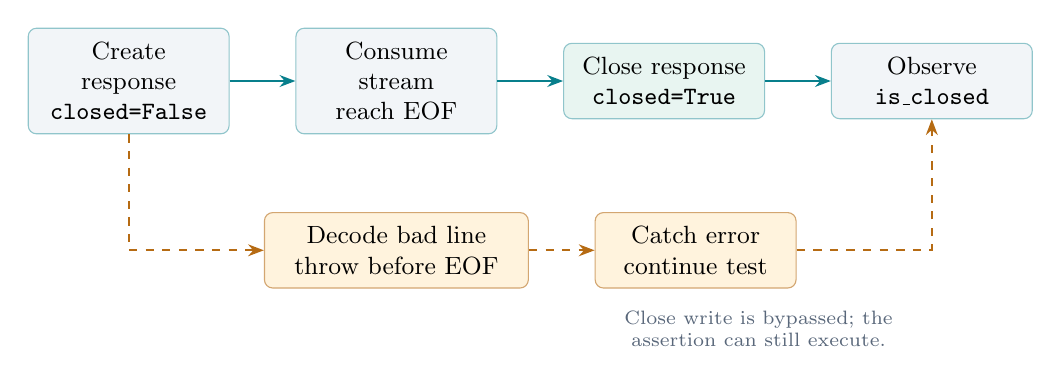
\begin{tikzpicture}
    \node[box,text width=2.2cm] (a) at (0,0) {Create response\\\code{closed=False}};
    \node[box,text width=2.2cm] (b) at (3.4,0) {Consume stream\\reach EOF};
    \node[box,fill=Mint,text width=2.2cm] (c) at (6.8,0) {Close response\\\code{closed=True}};
    \node[box,text width=2.2cm] (d) at (10.2,0) {Observe\\\code{is\_closed}};
    \draw[arrow] (a)--(b);\draw[arrow] (b)--(c);\draw[arrow] (c)--(d);
    \node[box,fill=Sand,draw=Amber!60,text width=3.0cm] (e) at (3.4,-2.15) {Decode bad line\\throw before EOF};
    \node[box,fill=Sand,draw=Amber!60,text width=2.2cm] (f) at (7.2,-2.15) {Catch error\\continue test};
    \draw[uncertain] (a.south) |- (e.west);
    \draw[uncertain] (e)--(f);
    \draw[uncertain] (f.east) -| (d.south);
    \node[labeltext,text width=4.0cm] at (8,-3.15) {Close write is bypassed; the assertion can still execute.};
  \end{tikzpicture}
  \takeaway{The same response and the observation after the exception matter. A malformed buffered JSON response may already be closed and reveal no defect.}
  \src{N01 candidate behavior and original trajectory. Arrows illustrate execution order; they do not claim a complete static proof.}
\end{frame}

% 5 ------------------------------------------------------------------------
\begin{frame}[t]{Four challenges determine whether a combination is useful}
  \begin{columns}[T,onlytextwidth]
    \begin{column}{.48\textwidth}
      \begin{block}{\faIcon{search}\quad Find the useful validation}
        Many temporary tests and variants compete for a small review budget. Historical tests may also become stale after later edits.
      \end{block}
      \begin{block}{\faIcon{link}\quad Connect the right context}
        Operations must concern the right object, input source and observation stage. Co-occurrence alone is insufficient.
      \end{block}
    \end{column}
    \begin{column}{.48\textwidth}
      \begin{block}{\faIcon{eye}\quad Make interaction observable}
        Inputs must change what the assertion can see. One-field schemas or normal completion can hide the interaction.
      \end{block}
      \begin{block}{\faIcon{balance-scale}\quad Keep a correct oracle}
        A combined context can invalidate old expectations. The submitted implementation may be wrong, so its output is not ground truth.
      \end{block}
    \end{column}
  \end{columns}
  \src{Observed across 17 development trials: N01 exception timing; N09 partial defaults; N05 oracle interpretation; N06 historical validation recovery.}
\end{frame}

% 6 ------------------------------------------------------------------------
\begin{frame}[t]{Core abstraction: the production path of an observation}
  \small\textbf{Unit:} an assertion on a specific object at a specific execution stage, together with the operations producing its observed value.
  \vspace{2mm}\centering
  \begin{tikzpicture}
    \node[box,text width=2.5cm] (a) at (0,0) {Input\\object state\\\faIcon{sliders-h}};
    \node[box,text width=3.5cm] (b) at (4.3,0) {Calls, branches and writes\\\faIcon{code-branch}};
    \node[box,text width=2.7cm] (c) at (8.8,0) {Assertion observation\\\faIcon{eye}};
    \draw[arrow] (a)--(b);\draw[arrow] (b)--(c);
    \node[box,fill=Lavender,draw=Purple!50,text width=3.5cm] (e) at (4.3,-1.8) {Edit an input\\or operation};
    \draw[arrow,draw=Purple] (e)--(b);
  \end{tikzpicture}
  \par\vspace{1mm}
  \begin{columns}[T,onlytextwidth]
    \begin{column}{.48\textwidth}\small\textbf{Search question}\par Can an edit change how this state is produced, while keeping the observation reachable?\end{column}
    \begin{column}{.48\textwidth}\small\textbf{Semantic question}\par What should hold in the new context, according to the issue and API contract?\end{column}
  \end{columns}
  \src{Research abstraction; bounded pieces are implemented. It is not a complete dependence model or a unified composition algorithm.}
\end{frame}

\begin{frame}[t]{Why an observation path helps expose a missing interaction}
  \begin{columns}[T,onlytextwidth]
    \begin{column}{.31\textwidth}
      \begin{block}{\faIcon{link}\quad Executable context}
        Reuse source inputs and calls; align their arguments and receiver objects.
      \end{block}
      \small\textbf{N01:} malformed bytes enter the same live response whose close state is checked.
    \end{column}
    \begin{column}{.31\textwidth}
      \begin{block}{\faIcon{eye}\quad Visible interaction}
        Trace the operations producing the observed value, including its stage.
      \end{block}
      \small\textbf{N09:} read the omitted default fields in the pending record, before flush.
    \end{column}
    \begin{column}{.31\textwidth}
      \begin{block}{\faIcon{balance-scale}\quad Contract reasoning}
        Provide relevant source facts; decide whether every expectation still holds.
      \end{block}
      \small\textbf{Both:} existing close/default expectations remain correct and expose the defect.
    \end{column}
  \end{columns}
  \takeaway{Analysis organizes the relevant program facts; the model reasons about a concrete combination and its complete expected behavior.}
  \src{This explains the mechanism in two confirmed examples. It is not a completeness or generalization guarantee.}
\end{frame}

% 7 ------------------------------------------------------------------------
\begin{frame}[t]{Overall workflow: source structure narrows semantic reasoning}
  \centering
  \begin{tikzpicture}
    \node[box,text width=3.5cm,minimum height=1.1cm] (a) at (0,0) {\faIcon{history}\quad Recover\\tests and source};
    \node[box,text width=3.5cm,minimum height=1.1cm] (b) at (4.25,0) {\faIcon{puzzle-piece}\quad Compose\\bounded source edits};
    \node[box,text width=3.5cm,minimum height=1.1cm] (c) at (8.5,0) {\faIcon{project-diagram}\quad Rank\\observation paths};
    \node[box,fill=Lavender,draw=Purple!50,text width=3.5cm,minimum height=1.1cm] (d) at (8.5,-1.8) {\faIcon{robot}\quad LLM review\\context + expectations};
    \node[box,text width=3.5cm,minimum height=1.1cm] (e) at (4.25,-1.8) {\faIcon{vial}\quad Execute\\controls and new tests};
    \node[box,fill=Mint,text width=3.5cm,minimum height=1.1cm] (f) at (0,-1.8) {\faIcon{clipboard-check}\quad Evaluate\\independent review};
    \draw[arrow] (a)--(b);\draw[arrow] (b)--(c);\draw[arrow] (c)--(d);
    \draw[arrow] (d)--(e);\draw[arrow] (e)--(f);
  \end{tikzpicture}
  \par\vspace{2mm}
  \small\textbf{Iteration:} preserve unserved candidates; expand the source frontier.\par
  \vspace{1mm}\textbf{Next:} use valid failures for patch repair and hidden-test evaluation.
  \src{Scored v3 uses existing writer/impact scheduling. The newer patch-to-observation ranking is a separate optional prototype.}
\end{frame}

% 8 ------------------------------------------------------------------------
\begin{frame}[t]{How existing tests become executable combination candidates}
  \small
  Parse tests and assertion APIs from repository and trajectory artifacts. Preserve their definitions, calls, fixtures and imports.
  \vspace{1mm}
  \begin{columns}[T,onlytextwidth]
    \begin{column}{.48\textwidth}
      \begin{block}{Source-derived building blocks}
        \begin{itemize}
          \item Inputs and argument positions.
          \item Calls, bindings and object reuse.
          \item Assertions and required execution prefixes.
        \end{itemize}
      \end{block}
      Finite edits: parameter replacement, operation composition, shared-object binding and field-presence changes.
    \end{column}
    \begin{column}{.48\textwidth}
      \begin{block}{N01: reuse two existing contexts}
        \textbf{Streaming test:}\par live response + close observation\par\vspace{2mm}
        \textbf{Error test:}\par malformed NDJSON + decoding-error check\par\vspace{2mm}
        \textbf{Combination:}\par malformed input in the live response; observe close after catching the error.
      \end{block}
    \end{column}
  \end{columns}
  \src{Executability does not establish semantic correctness. Deriving new edits directly from paths remains open.}
\end{frame}

% 9 ------------------------------------------------------------------------
\begin{frame}[t,fragile]{Latest ranking prototype: distinguish edits inside the same test}
  \begin{columns}[T,onlytextwidth]
    \begin{column}{.45\textwidth}
      \begin{lstlisting}[language=Python]
# Submitted patch changed this return.
def calculate(value, unused):
    return value * 3

result = calculate(1, 10)
assert result == 3
      \end{lstlisting}
      \small\textbf{Candidate A:} change \code{1} to \code{2}.\\
      \textbf{Candidate B:} change \code{10} to \code{11}.
    \end{column}
    \begin{column}{.51\textwidth}
      \begin{block}{Candidate-conditioned dependency}
        Both candidates call the modified function. Only A's edited argument participates in the return value seen by the assertion.
      \end{block}
      \small\textbf{Strict:} project arguments through finite return dependencies.\\[1.5mm]
      \textbf{May:} use a conservative same-call path to a modified callee; may include unused arguments.
    \end{column}
  \end{columns}
  \takeaway{Reparse the edited test and join at the same call site. A missing path remains unknown.}
  \src{Illustrative fixture; not a DeepSWE result. The optional ranking prototype's full comparison is pending.}
\end{frame}

% 10 -----------------------------------------------------------------------
\begin{frame}[t]{The LLM gets one concrete semantic task}
  \begin{columns}[T,onlytextwidth]
    \begin{column}{.48\textwidth}
      \begin{block}{\faIcon{file-code}\quad Program-produced evidence}
        \begin{itemize}
          \item Fixed input/operation edits.
          \item Complete test and all assertions.
          \item Calls, arguments and source bodies.
          \item Issue contract and analysis unknowns.
        \end{itemize}
      \end{block}
    \end{column}
    \begin{column}{.48\textwidth}
      \begin{block}{\faIcon{robot}\quad Semantic decision}
        Is this a legal context? Which expectations remain valid? What should replace the expectations that change?
      \end{block}
      \small Output: retain, revise, or unknown. Code applies supported edits to expectations, preserving actions and observations.
    \end{column}
  \end{columns}
  \takeaway{Infer expectations from the contract, not the buggy output. Review all assertions and prerequisites.}
  \src{Completed v3: at most 16 semantic candidates per trial per round; one full candidate per request; fresh DeepSeek-v4-flash requests.}
\end{frame}

% 11 -----------------------------------------------------------------------
\begin{frame}[t]{Formal problem: find a valid defect-exposing combined context}
  \small Input: candidate program $P$, issue contract $I$, repository $R$, original trajectory $H$, and budgets $B$.
  \vspace{2mm}
  \[
    T_0=\operatorname{Extract}(R,H),\qquad
    \mathcal{C}=\{\operatorname{Apply}(t,\delta)\mid t\in T_0,\ \delta\in\mathcal{E}(T_0,R)\}.
  \]
  \small $T_0$: recovered tests; $\mathcal{E}$: finite input/operation edits; $\mathcal{C}$: combined contexts before oracle review.
  \begin{block}{Search objective}
    Find $c\in\mathcal{C}$ and reviewed expectations $o$. Materialize $u=\operatorname{Test}(c,o)$ such that:
    \[
      \operatorname{Valid}_{I}(u)\ \land\
      \bigwedge_{s\in\operatorname{Controls}(u)}\operatorname{Pass}(P,s)\ \land\
      \operatorname{IssueFail}_{I}(P,u).
    \]
  \end{block}
  \small\textbf{Valid}: legal test and correct complete expectations. \textbf{Controls}: associated source tests. \textbf{IssueFail}: confirmed issue-related failure, including a defect-induced panic.
  \src{Independent semantic review; compile/environment errors excluded. Budgets limit composition, requests and execution.}
\end{frame}

\begin{frame}[t]{Formal success criterion: a valid, issue-related native failure}
  \begin{columns}[T,onlytextwidth]
    \begin{column}{.48\textwidth}
      \begin{block}{$\operatorname{Valid}_I(u)$: semantic validity}
        Legal setup, meaningful observations and correct complete expectations, including assertions before the final observation.
      \end{block}
      \begin{block}{$\operatorname{Pass}(P,s)$: source control}
        Associated original tests pass on the same replayed candidate program.
      \end{block}
    \end{column}
    \begin{column}{.48\textwidth}
      \begin{block}{$\operatorname{IssueFail}_I(P,u)$: defect evidence}
        Confirmed issue-related native test failure: an assertion mismatch or a defect-induced exception/panic under valid setup.
      \end{block}
      \small Compile and environment errors do not qualify. Semantic validity is assessed independently; our analyzer does not prove it.
    \end{column}
  \end{columns}
  \takeaway{The defect escaped effective pre-submission validation. Its combined relation need not be absent from every earlier trajectory step.}
  \src{N06 recovers a historical combination not revalidated on the final patch. P5 exposes a defect-induced VM panic before later assertions.}
\end{frame}

% 12 -----------------------------------------------------------------------
\begin{frame}[t]{Formal abstraction: edits, production paths and observations}
  \small For an edited test $u$, construct a bounded dependence graph $G_u=(V_u,E_u)$ from the actual edited source.
  \vspace{1mm}
  \begin{columns}[T,onlytextwidth]
    \begin{column}{.48\textwidth}
      \begin{block}{Computable components}
        \begin{itemize}
          \item $D_u$: input/operation edit nodes.
          \item $\Delta$: modified production code.
          \item $a_q$: actual-value node of assertion $q$.
          \item Edges: value, control, supported calls/effects.
        \end{itemize}
      \end{block}
    \end{column}
    \begin{column}{.48\textwidth}
      \begin{block}{Path-relevance query}
        \[
          d\in D_u\ \leadsto\ p\in\Delta\ \leadsto\ a_q
        \]
        $\leadsto$: supported dependence reachability. Join compatible bindings at the \textbf{same statically identified call site}.
      \end{block}
      \small N01: malformed bytes affect decoding; an exception bypasses the observed close write.
    \end{column}
  \end{columns}
  \small\textbf{Limit:} a path helps reasoning; it does not prove feasibility, oracle correctness or complete coverage.
  \src{Bounded research definition; heap/exception modeling is incomplete and differs across implemented modules.}
\end{frame}

% 13 -----------------------------------------------------------------------
\begin{frame}[t]{Formal method: stable path priority, bounded oracle review}
  \small Let $F$ be the deterministic family/seed/shape order of the fixed candidate pool.
  \begin{block}{Two predeclared path predicates}
    \small $S(u)$: an edited input reaches modified code through supported return dependencies and then the actual observation.\\[1mm]
    $M(u)$: an edited input affects a concrete call in the actual-value slice; its reliable callee can reach modified code. This is weaker may evidence.
  \end{block}
  \[
    \operatorname{Rank}_{m}(F)=
    [u\in F\mid m(u)]\ \mathbin{\Vert}\ [u\in F\mid\neg m(u)],\quad m\in\{S,M\}.
  \]
  \small $\Vert$: concatenation; partitions preserve $F$'s order. Fallback includes unsupported and unknown candidates.
  \vspace{2mm}
  \small\textbf{Review:} select up to $B_o$ requestable, unserved candidates per round; infer expectations and execute. $B_o$ is the semantic budget. Keep pending candidates.
  \src{Latest optional strict/may ranking and CLI. The frozen 16/17 run used earlier writer/impact scheduling; no result is attributed to this new rule.}
\end{frame}

% 14 -----------------------------------------------------------------------
\begin{frame}[t,fragile]{N01 worked example: the combined test checks close after failure}
  \begin{columns}[T,onlytextwidth]
    \begin{column}{.59\textwidth}
      \begin{lstlisting}[language=Python]
def chunks():
    yield b'{"a": 1}\nnot json\n'
    yield b'1}'  # unread when parsing fails

response = httpx.Response(
    200,
    headers={"Content-Type":
             "application/x-ndjson"},
    stream=IteratorByteStream(chunks()),
)
with pytest.raises(httpx.DecodingError):
    list(response.iter_json())
assert response.is_closed
      \end{lstlisting}
      \scriptsize Executed witness condensed: imports, names and additional checks omitted here.
    \end{column}
    \begin{column}{.37\textwidth}
      \begin{block}{Why this input works}
        A malformed complete line is parsed while the stream is live. Catch the error, then observe close.
      \end{block}
      \small\textbf{Contract:} close after streaming consumption.\\[1.5mm]
      \textbf{Required:} \code{True}.\\
      \textbf{Candidate returns:} \code{False}.\\[1.5mm]
      The original close oracle is retained.
    \end{column}
  \end{columns}
  \src{Executed N01 witness \code{c8e075c82686eb21c4222575}; source and native execution in the v3 ledger.}
\end{frame}

% 15 -----------------------------------------------------------------------
\begin{frame}[t]{N01 worked example: evidence from recovery to native failure}
  \renewcommand{\arraystretch}{1.06}
  \small
  \begin{tabular}{@{}L{.19\textwidth}L{.73\textwidth}@{}}
    \toprule
    Stage & What actually happened in the completed v3 run\\\midrule
    Recover & Stream construction and close checks; malformed donor input and error handling.\\
    Compose & Align the response; transfer input, header and exception context into its live generator.\\
    Select/review & Exception/write context informs priority; retain the original close oracle.\\
    Execute & Source controls pass. Generated pytest test fails: \code{is\_closed} is \code{False}.\\
    Confirm & Independent evaluation checks the complete test, emitted source and native failure.\\\bottomrule
  \end{tabular}
  \takeaway{A complete native defect witness on the replayed submitted patch; the patch itself is not repaired.}
  \src{N01 deliveries and runtime index; main v3 \code{checkpoint\_14.json}.}
\end{frame}

% 16 -----------------------------------------------------------------------
\begin{frame}[t,fragile]{Second real success: Koota partial defaults before flush (N09)}
  \small\textbf{Contract:} deferred \code{get} must return the same logical values as after \code{flush}. A partial parameter object must retain omitted defaults.
  \begin{columns}[T,onlytextwidth]
    \begin{column}{.57\textwidth}
      \begin{lstlisting}[language=TypeScript]
// Existing Test fixture defaults include:
// current=1, test='hello', bool=true.
const entity = world.spawn();
world.deferred.add(entity,
  Test({current: 2, arr: ['d','e','f']}));
const test = entity.get(Test); // no flush
expect(test).toMatchObject({
  current: 2, test: 'hello', bool: true,
  arr: ['d','e','f']
});
      \end{lstlisting}
      \scriptsize Condensed executed witness; the complete original fixture, class/default checks and later actions are preserved in the actual test.
    \end{column}
    \begin{column}{.39\textwidth}
      \small\textbf{Recover:} repository test for ordinary partial \code{entity.add}.\\[2mm]
      \textbf{Compose:} replace that call with \code{world.deferred.add}; preserve bindings and expectations.\\[2mm]
      \textbf{Observe:} read before flush. The buggy projection returns supplied parameters without omitted defaults.\\[2mm]
      \yes\ Source control passes; generated Vitest test fails on missing defaults.
    \end{column}
  \end{columns}
  \src{Public \href{https://deepswe.datacurve.ai/data/v1.1/trials/koota-deferred-mutation-buffer__whVuJZW}{N09 trial}; main witness \code{08f2c625387570b30312}. Source expectations retained.}
\end{frame}

% 17 -----------------------------------------------------------------------
\begin{frame}[t]{Evaluation protocol: a confirmed witness, not any failing test}
  \begin{columns}[T,onlytextwidth]
    \begin{column}{.48\textwidth}
      \begin{block}{Completed main experiment}
        \begin{itemize}
          \item 17 trials, 14 distinct tasks.
          \item 7 original pilots + 10 Flash failures.
          \item All used during development.
          \item Frozen v3: \code{7a8ff95}; 2 rounds.
        \end{itemize}
      \end{block}
      \small Fresh oracle requests; original trajectories available. No prior-answer reuse.
    \end{column}
    \begin{column}{.48\textwidth}
      \begin{block}{Trial-level detection metric}
        Count a trial only with legal context, correct complete expectations, passing controls and a named issue-related failure.
      \end{block}
      \small\textbf{Separate metrics:} target exposure/rank, complete oracle correctness, execution errors, calls and tokens.
    \end{column}
  \end{columns}
  \takeaway{Rank, test correctness and issue resolution are different metrics. Overall false-positive rate is not yet established.}
  \src{v3 independent evaluation, \code{checkpoint\_14.json}. P1--P3 share a task; P5/P6 share another.}
\end{frame}

% 18 -----------------------------------------------------------------------
\begin{frame}[t]{All 17 trials: 16 confirmed witnesses, one remaining miss}
  \setlength{\tabcolsep}{3pt}
  \begin{columns}[T,onlytextwidth]
    \begin{column}{.47\textwidth}
      \small\textbf{Original seven pilots}\par\vspace{1mm}
      \scriptsize\renewcommand{\arraystretch}{1.20}
      \begin{tabular}{@{}llcl@{}}
        \toprule Case & Interaction & Hit & Oracle\\\midrule
        P1 & Textual: event phase & \yes & \Rev\\
        P2 & Textual: shortcut + text & \yes & \Ret\\
        P3 & Textual: shifted alias & \yes & \Ret\\
        P4 & IPython: quoted path & \yes & \Ret\\
        P5 & Tengo: returned callable & \yes & \Ret\\
        P6 & Tengo: shared cells & \yes & \Rev\\
        P7 & Valibot: recursive transform & \yes & \Rev\\\bottomrule
      \end{tabular}
      \par\vspace{2mm}
      \scriptsize Pilots have several original agent models. The ten added trials all use Flash.
    \end{column}
    \begin{column}{.50\textwidth}
      \small\textbf{Ten DeepSeek-v4-flash trials}\par\vspace{1mm}
      \scriptsize\renewcommand{\arraystretch}{1.12}
      \begin{tabular}{@{}llcl@{}}
        \toprule Case & Interaction & Hit & Oracle\\\midrule
        N01 & HTTPX: JSON error + close & \yes & \Ret\\
        N02 & HTTPX: multipart + close & \yes & \Ret\\
        N03 & mnamer: duplicate + quota & \yes & \Ret\\
        N04 & sqlite-utils: bulk + invariant & \yes & \Rev\\
        N05 & termenv: fitting + reset & \pending & --\\
        N06 & etree: sibling insert + text & \yes & \Ret\\
        N07 & go-git: overlapping edits & \yes & \Ret\\
        N08 & Pebble: exclusive frontier & \yes & \Ret\\
        N09 & Koota: partial defaults & \yes & \Ret\\
        N10 & DDBToolbox: omitted mode & \yes & \Ret\\\bottomrule
      \end{tabular}
    \end{column}
  \end{columns}
  \par\vspace{1mm}
  \scriptsize N06 recovers a historical relation; N07 uses an alternative witness; N08 uses new valid premises. DDBToolbox = DynamoDB Toolbox.
  \src{12 retained source oracles + 4 revised = 16 detected. All are development trials, not held-out generalization.}
\end{frame}

% 19 -----------------------------------------------------------------------
\begin{frame}[t]{Results: practical progress with limited causal evidence}
  \begin{columns}[T,onlytextwidth]
    \begin{column}{.47\textwidth}
      \begin{block}{Completed main run}
        \centering\vspace{2mm}{\Huge\textcolor{Teal}{16}/17}\par
        \small Confirmed development-trial witnesses\par\vspace{2mm}
        
\begin{tikzpicture}
          \fill[Teal] (0,0) rectangle (4.7,.32);
          \fill[Amber] (4.7,0) rectangle (5.0,.32);
        \end{tikzpicture}\par
        \small 540 fresh calls; 7.42M total tokens.\par
        83 responses reached the output limit.
      \end{block}
    \end{column}
    \begin{column}{.49\textwidth}
      \begin{block}{Isolated local evidence}
        Same eight Python pools, eight proposals each, no LLM: writer-path static priority improved confirmed detection \textbf{3/8 $\rightarrow$ 4/8}.
      \end{block}
      \small Added N01. This supports a local search rule, not a universal abstraction.\\[2mm]
      Earlier 12/17 and current 16/17 use different configurations; their difference does not isolate the analysis contribution.
    \end{column}
  \end{columns}
  \src{Main score: v3 checkpoint 14 and provider receipts. Local equal-budget experiment: assertion-writer search report. Tokens include reasoning once.}
\end{frame}

% 20 -----------------------------------------------------------------------
\begin{frame}[t]{Academic novelty: a contribution hypothesis with a clear boundary}
  \small\textbf{Candidate insight:} search for edits affecting one observation's production path; ask the model only about the remaining contract semantics.
  \vspace{1mm}\renewcommand{\arraystretch}{1.0}
  \small
  \begin{tabular}{@{}L{.28\textwidth}L{.63\textwidth}@{}}
    \toprule Design element & Current academic assessment\\\midrule
    Candidate-specific query & Joins edit, patch and observation at one call site. Its precision benefit is unverified.\\
    Classical analysis & Slicing, binding, return summaries and call graphs are established.\\
    Analysis + LLM & Precedent in STARS; this division alone is not novel.\\
    Missing capability & A unified path-driven synthesis operator: paths currently rank existing candidates.\\\bottomrule
  \end{tabular}
  \takeaway{Hypothesis to test: observation-driven search improves valid defect detection at equal budget.}
  \src{Not a demonstrated unified innovation. STARS, ChaCo and Testora supply relevant baselines; see references.}
\end{frame}

% 21 -----------------------------------------------------------------------
\begin{frame}[t]{Current limitations: selection, oracle reliability and analysis cost}
  \begin{columns}[T,onlytextwidth]
    \begin{column}{.48\textwidth}
      \begin{alertblock}{N05: an unresolved complete witness}
        Fitting width + preserve reset. Target ranks \textbf{96 and 122} in the two rounds; never offered. A related executed variant kept an invalid truncation expectation.
      \end{alertblock}
      \small Both budget allocation and complete oracle inference remain bottlenecks.
    \end{column}
    \begin{column}{.48\textwidth}
      \begin{alertblock}{Source-analysis prototype is costly}
        A 370-candidate Go pool took \textbf{33.2 minutes} in strict mode, also computing may evidence. This is whole-pool cost.
      \end{alertblock}
      \small Helper, heap, callback and scope support is incomplete. The new 17-trial ranking census is still pending.
    \end{column}
  \end{columns}
  \takeaway{34 sampled raw failures: 30 invalid tests, 2 valid detections, 2 uncertain contracts. This is not the overall false-positive rate.}
  \src{N05 final audit; independent failure sample; patch-priority v1 census, P5 strict = 1990.317 seconds. No new ranking/detection gain is claimed.}
\end{frame}

% 22 -----------------------------------------------------------------------
\begin{frame}[t]{Next research steps: make the abstraction drive synthesis}
  \begin{columns}[T,onlytextwidth]
    \begin{column}{.48\textwidth}
      \begin{block}{\faIcon{puzzle-piece}\quad Path-driven composition}
        Derive new edits from paths, beyond current constructors. Compare under equal budgets.
      \end{block}
      \begin{block}{\faIcon{eye}\quad Complete observations}
        Preserve object identity, phases and prerequisites. Audit every assertion against contract evidence.
      \end{block}
    \end{column}
    \begin{column}{.48\textwidth}
      \begin{block}{\faIcon{tachometer-alt}\quad Bounded analysis cost}
        Index assertions and cache call facts. Measure whole-pool and online latency.
      \end{block}
      \begin{block}{\faIcon{flask}\quad Independent evaluation}
        Freeze unseen trials; repeat model runs; evaluate repair with hidden tests.
      \end{block}
    \end{column}
  \end{columns}
  \takeaway{Success: more valid witnesses and better repaired patches at fixed total budget, with measured misses and false alarms.}
  \src{Planned work. Current evidence establishes local detection progress, not zero false negatives, generality, or issue-resolution improvement.}
\end{frame}

\appendix
\section*{References and Evidence}

% 23 -----------------------------------------------------------------------
\begin{frame}[t]{Reference points for the research design}
  \small
  \begin{itemize}
    \item \href{https://software-lab.org/publications/issta2026_STARS.pdf}{\textbf{STARS, ISSTA 2026}}: static analysis synthesizes assertion components, including type-connected observer call chains; LLMs concretize assertions.
    \item \href{https://software-lab.org/publications/icse2026_ChaCo.pdf}{\textbf{Change And Cover, ICSE 2026}}: patch-focused regression-test augmentation and recovery of project-specific test context; assumes a bug-free PR.
    \item \href{https://software-lab.org/publications/icse2026_Testora.pdf}{\textbf{Testora, ICSE 2026}}: compares pre/post-change behavior and uses documented change intent to classify differences.
    \item \href{https://conf.researchr.org/details/issta-2026/issta-2026-research-papers/123/Towards-More-Realistic-Assertion-Generation-under-Mixed-Assertion-Scenario}{\textbf{Mixed-Assertion Scenario, ISSTA 2026}}: multiple assertions jointly express test objectives; known insertion positions are a consequential assumption.
  \end{itemize}
  \takeaway{Our comparison must isolate candidate composition, observation relevance and oracle correctness. Classical analysis and context retrieval are strong baselines.}
  \src{Primary author papers and official conference abstract. These comparisons motivate design choices; they do not establish global novelty.}
\end{frame}

% 24 -----------------------------------------------------------------------
\begin{frame}[t]{Evidence map and reproducible scope}
  \small
  \begin{tabular}{@{}L{.22\textwidth}L{.70\textwidth}@{}}
    \toprule Material & Repository-relative location\\\midrule
    Current method & \path{research/method_design.md}\\
    Original trials & \path{research/expanded_trials_20260926/cases.json};\\
      & \path{data/relational_gap_v1/N01/trajectory.json}; N09 likewise\\
    Main score & \path{results/relation_search_20260929_v3/evaluation/}\\
      & \path{uniform_fresh_impact_v3/checkpoint_14.json}\\
    Native witnesses & Same directory: N01 deliveries and N09 runtime index\\
    Implementation & \path{relation_search/}; \path{scripts/run_relation_campaign.py}\\
    New ranking & \path{experimental/patch_observation_priority.py}\\
    This presentation & \path{docs/combination_testing_research.tex}\\\bottomrule
  \end{tabular}
  \par\vspace{2mm}
  \small\textbf{Frozen distinction:} scored v3 is \code{7a8ff95}; later source-priority integration is \code{7615f4e}. New prototype results do not overwrite the scored run.
  \src{Report snapshot: 30 September 2026. Public issue/trajectory/patch evidence; no hidden verifier or reference patch is used for generation.}
\end{frame}

\end{document}
